\subsection{Mobile Network Transitions}
\label{subsec-networktransitions}

Mobile devices like smartphones move through a complex network environment.
Providing the illusion of seamless connectivity requires negotiating hand-offs
both between WiFi access points and between WiFi and 3G radios. Further
exacerbating the situation, users are typically very aware of the device's
mistakes. It is clear to them that the phone should give up on the WiFi
signal since they are halfway across the parking lot. Unfortunately, it is
not so obvious to Android.

\begin{figure*}[t]
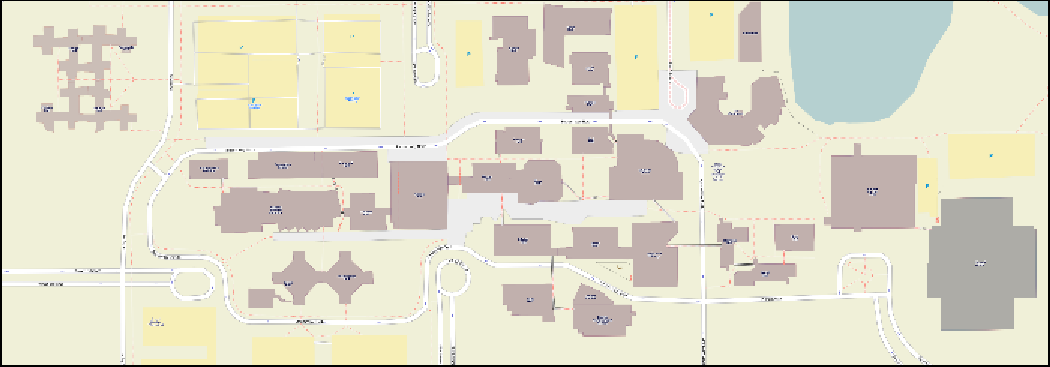
\includegraphics[width=\textwidth]{./figures/networking/transition_locations/graph.pdf}
\caption{\textbf{3G to WiFi transition locations.} The map indicates that
there are several common areas where network hand-offs occur.}
\label{figure-networktransitions}
\end{figure*}

\subsubsection{Stuck in the middle}

We were interested in observing hand-offs between 3G and WiFi and found many
in the dataset collected by our usage experiment. Since the Android
\texttt{ConnectivityService} frequently switches network interfaces for
exploration purposes, we have defined a transition as two one-minute or
longer sessions on different interfaces separated by less than one minute. We
further limit ourselves to cases where we received a location update during
the transition.

Figure~\ref{figure-networktransitions} plots the location of transitions that
occurred on or near SUNY North Campus. We notice that many cluster in
expected locations: near the entrance and exits of buildings where
participants are likely to be moving from campus WiFi to Sprint 3G.

\subsubsection{Future experiments}

Mapping and remembering where network transitions take place may allow the
Android platform to conduct the transitions more smoothly. When it observes a
participant heading towards a transition area, it may decide to be more
aggressive about abandoning the current interface and less inclined to hang on
to a weakening connection. Platform experiments using transition data
generated by \PhoneLab{} participants would use this crowd-sourced transition
map to adjust the policies of the \texttt{ConnectivityService} component.
Improvements in hand-offs could be benchmarked against unmodified \PhoneLab{}
phones.
